\documentclass[11pt]{article}

\usepackage{amsmath,amssymb,amsfonts}
\usepackage{graphicx}
\usepackage{pgfplots}
\usepackage{multicol}
\usepackage{enumitem}
\usepgfplotslibrary{fillbetween}
\pgfplotsset{compat=1.16,width=10cm}


\setlength{\topmargin}{-.5in} \setlength{\textheight}{9.25in}
\setlength{\oddsidemargin}{0in} \setlength{\textwidth}{6.8in}


\begin{document}

\Large

\noindent{\bf Name: \hfill Date: \hfill Quiz 5 \hfill Precalculus - Hargus}

\medskip\hrule
\vspace{10pt}

\noindent \textbf{Instructions:} Please \textbf{show all work} (partial credit will be given for correct work, even if your answer is wrong).

\vspace{10pt}

\begin{enumerate}

\item (15 points) Let $\textbf{u}= \langle 5,3 \rangle$ and $\textbf{v}=\langle -1,2 \rangle$. Write your answers in component form.

\begin{enumerate}[itemsep=10pt, label={\alph*)}]
    \item $\displaystyle 3\textbf{v} = $
    \item $\displaystyle \textbf{u} + 2\textbf{v} = $
    \item $\displaystyle \textbf{u} \cdot \textbf{v} = $
\end{enumerate}
\vspace{10pt}

\item (5 points) Find the angle between the vectors $\textbf{u}= \langle 5,3 \rangle$ and $\textbf{v}=\langle -1,2 \rangle$.
\vspace{60pt}
\begin{flushright}
Angle $= \rule{3cm}{0.4pt}$
\end{flushright}

\vspace{10pt}

\item (10 points) Eliminate the parameter $t$ from the following parametric equations. For your answer, write $y$ in terms of $x$.

\begin{enumerate}[itemsep=20pt, label={\alph*)}]
\item $x = t - 1$ \\
$y = t^2 +4t$
\vspace{50pt}
\begin{flushright}
$y = \rule{4cm}{0.4pt}$
\end{flushright}
\item $x = 3\cos(t)$ \\
$y = 3\sin(t)$
\vspace{50pt}
\begin{flushright}
$y = \rule{4cm}{0.4pt}$
\end{flushright}
\end{enumerate}

\item (15 points) Steven shoots and makes a basket from a horizontal distance of $d = 10$ ft from a basketball hoop. The basketball has initial velocity $v_0 = 20$ ft/s and an initial angle of $\theta = 50^{\circ}$. 

%\includegraphics[width = .45\linewidth]{basketball}


\begin{center}


\tikzset{every picture/.style={line width=0.75pt}} %set default line width to 0.75pt        

\begin{tikzpicture}[x=0.75pt,y=0.75pt,yscale=-1,xscale=1]
%uncomment if require: \path (0,300); %set diagram left start at 0, and has height of 300

%Shape: Circle [id:dp5310262351368967] 
\draw   (162,123) .. controls (162,117.48) and (166.48,113) .. (172,113) .. controls (177.52,113) and (182,117.48) .. (182,123) .. controls (182,128.52) and (177.52,133) .. (172,133) .. controls (166.48,133) and (162,128.52) .. (162,123) -- cycle ;
%Straight Lines [id:da8244021660122901] 
\draw [line width=2.25]    (177,114) -- (213.84,55.24) ;
\draw [shift={(216.5,51)}, rotate = 482.09] [fill={rgb, 255:red, 0; green, 0; blue, 0 }  ][line width=0.08]  [draw opacity=0] (14.29,-6.86) -- (0,0) -- (14.29,6.86) -- cycle    ;
%Shape: Ellipse [id:dp8104144019867403] 
\draw  [line width=1.5]  (318,44.5) .. controls (318,41.46) and (325.28,39) .. (334.25,39) .. controls (343.22,39) and (350.5,41.46) .. (350.5,44.5) .. controls (350.5,47.54) and (343.22,50) .. (334.25,50) .. controls (325.28,50) and (318,47.54) .. (318,44.5) -- cycle ;
%Straight Lines [id:da3732141641924541] 
\draw [line width=2.25]    (365.5,39) -- (365.5,187) ;
%Straight Lines [id:da2856435588909767] 
\draw [line width=2.25]    (351.5,27) -- (365.5,39) ;
%Straight Lines [id:da8676014399053691] 
\draw [line width=2.25]    (351.5,18) -- (351.5,52) ;
%Straight Lines [id:da325740426596309] 
\draw    (172,123) -- (333.5,123) ;
%Straight Lines [id:da4350954289209674] 
\draw  [dash pattern={on 4.5pt off 4.5pt}]  (334.25,36) -- (333.5,123) ;
%Curve Lines [id:da5707969445007132] 
\draw    (187,102) .. controls (195.5,105) and (200.5,115) .. (197.5,124) ;
%Straight Lines [id:da1572576439170188] 
\draw    (152.5,143) -- (152.5,169) ;
%Straight Lines [id:da4070068592272875] 
\draw    (164.5,131) -- (152.5,143) ;
%Straight Lines [id:da846513392557126] 
\draw    (152.5,169) -- (160.5,186) ;
%Straight Lines [id:da9556654767114634] 
\draw    (152.5,169) -- (146.5,186) ;
%Straight Lines [id:da33603862330138934] 
\draw    (152.5,143) -- (152.5,135) ;
%Shape: Circle [id:dp092422308104808] 
\draw   (145.5,128) .. controls (145.5,124.13) and (148.63,121) .. (152.5,121) .. controls (156.37,121) and (159.5,124.13) .. (159.5,128) .. controls (159.5,131.87) and (156.37,135) .. (152.5,135) .. controls (148.63,135) and (145.5,131.87) .. (145.5,128) -- cycle ;

% Text Node
\draw (189,33.4) node [anchor=north west][inner sep=0.75pt]  [font=\large]  {$\overrightarrow{v_{0}}$};
% Text Node
\draw (254.75,126.4) node [anchor=north west][inner sep=0.75pt]    {$d$};
% Text Node
\draw (319,73.4) node [anchor=north west][inner sep=0.75pt]    {$h$};
% Text Node
\draw (199,96.4) node [anchor=north west][inner sep=0.75pt]    {$\theta $};

\end{tikzpicture}
\end{center}



\begin{enumerate}[itemsep=10pt, label={\alph*)}]
\item What is the component of the initial velocity in the vertical y-direction $v_{0_y}$?
\vspace{40pt}
\begin{flushright}
$v_{0_y}$= $\rule{3cm}{0.4pt}$
\end{flushright}
\item After what length of time $t$ has the ball traveled a horizontal distance of $d = 10$ ft?
\vspace{80pt}
\begin{flushright}
$t= \rule{3cm}{0.4pt}$
\end{flushright}
\item What is the height $h$ of the basketball above where it was shot (see diagram above) at the time $t$ you found in part (b)? Hint: remember that the height of a flying object is given by $y = -16 t^2 + v_{0_y}t + y_0$.
\vspace{100pt}
\begin{flushright}
$h = \rule{3cm}{0.4pt}$
\end{flushright}
\end{enumerate}

\newpage

\item (5 points) Convert the equation $r \sec(\theta) = 3$ to rectangular form (using only $x$ and $y$). Write your answer in the standard form for a circle $(x-a)^2 + (y-b)^2 = c^2$, where $a$, $b$, and $c$ are constants. 

\vspace{200pt}
\begin{flushright}
Rectangular form: $\rule{5cm}{0.4pt}$
\end{flushright}

\vspace{20pt}
\item (5 points) Show that the graph of the polar equation $r = 1 + 2\cos(\theta)$ is symmetric across the $x$-axis, using a symmetry test.
\vspace{180pt}

\newpage

\item (10 points) True or false? (circle your answer)
\begin{enumerate}[itemsep=15pt, label={\alph*)}]
\item If \textbf{u} and \textbf{v} are vectors, then $\textbf{u} \cdot \textbf{v} =  \textbf{v} \cdot \textbf{u}$ \null\hfill \textbf{T} or \textbf{F}
\item If \textbf{u} and \textbf{v} are vectors, then $|\textbf{u}| |\textbf{v}| =  \textbf{u} \cdot \textbf{v}$  \null\hfill \textbf{T} or \textbf{F}
\item If \textbf{u} and \textbf{v} are nonzero vectors, then \textbf{u} and \textbf{v} are parallel if and only if $\textbf{u} \cdot \textbf{v} = 0$.  \null\hfill \textbf{T} or \textbf{F}
\item The polar coordinates $(2, -\frac{\pi}{2})$ and $(-2, \frac{5\pi}{2})$ are the same point. \\ \null\hfill \textbf{T} or \textbf{F}
\item The distance between any two points in polar coordinates $(r_1, \theta_1)$ and $(r_2, \theta_2)$ is $|r_1 - r_2|$. \null\hfill \textbf{T} or \textbf{F}
\end{enumerate}

\vspace{20pt}

\item (10 points) The graph of $r = 5\sin(2\theta) + 1$ is shown below. What are the lengths of the petals $l_1$ and $l_2$?

\begin{center}
\begin{tikzpicture}
  \draw[thick,->,>=latex] (-3,0)--(3,0) node[above] {$x$};
  \draw[thick,->,>=latex] (0,-3)--(0,3) node[left] {$y$};
  \draw[thick,-,>=latex] (0,0)--(2.54,2.54) node[pos=0.5, above] {$l_2$};
  \draw[thick,-,>=latex] (0,0)--(-1.697,1.697) node[pos=0.5, above] {$l_1$};
  \draw[domain=0:540,scale=.6,samples=500] plot (\x:{5*sin(2*\x)+1});
\end{tikzpicture}
\end{center}

\vspace{50pt}

\begin{flushright}
$l_1$= $\rule{3cm}{0.4pt}$
\end{flushright}

\begin{flushright}
$l_2$= $\rule{3cm}{0.4pt}$
\end{flushright}

\end{enumerate}

\end{document} 